\section{Programming: Least Squares Regression } 

\subsection {Data Set 1 (synthetic 1-dimensional data)} This data set contains 100 training examples and 1000 test examples, all generated i.i.d. from a fixed probability distribution. For this data set, you will run unregularized least squares regression.

    \begin{enumerate}
    
        \item \textbf{Learning Curve.} 
        \begin{figure}[H]
            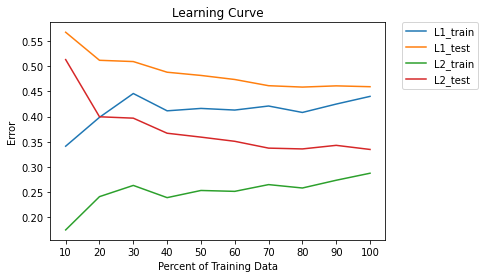
\includegraphics[scale=0.5, angle=0]{templates/1_1_1.png}
            \centering
            \caption{Curves showing $L1$ and $L2$ errors as a function of number of training samples used.}
            \label{fig:my_label}
        \end{figure}
        
        \item \textbf{Analysis of model learned from full training data.} 
        
        \begin{figure}[H]
            \centering
            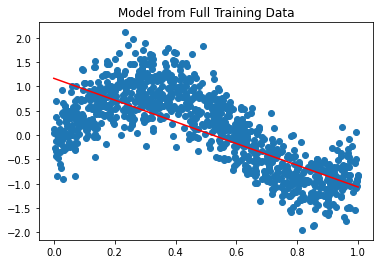
\includegraphics[scale=0.5, angle=0]{templates/1_1_2.png}
            \caption{Plot of learned linear function and scatter plot depicting true test labels.}
            \label{fig:my_label}
        \end{figure}
        
        \begin{verbatim}
        w:  [[-2.23442304]]
        b:  1.1671738819238153
        L2 training error: 0.2876339586619919
        L2 test error    : 0.33475968697353337
        \end{verbatim}
    \end{enumerate}
    
\subsection {Data Set 2 (real 8-dimensional data)} This is a real data set that involves predicting median house value from the location coordinates, demographics and the number of rooms and bedrooms in the houses in total in the block (or district). The data set is a subset of a larger dataset curated for a research conducted by Pace,R. Kelly and Ronald Barry in 1997.This subset has 960 training examples and 240 test examples. For this data set, you will run both unregularized least squares regression and $L_2$-regularized least squares regression (ridge regression).
    
    \begin{enumerate}
        \item \textbf{Regression on 5$\%$ of the training data.} 
        
        \begin{figure}[H]
            \centering
            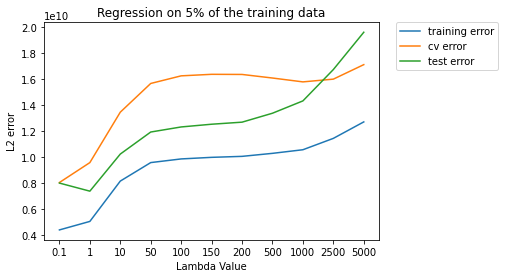
\includegraphics[scale=0.5, angle=0]{templates/1_2_1.png}
            \caption{Plot showing $\lambda$ and cross-validation loss.}
            \label{fig:my_label}
        \end{figure}
        
        \begin{verbatim}
            lambda:  0.1  
            b:  -3064.11067472829
            w: [ [ 3.38723280e+03]
                 [ 7.58457227e+03]
                 [ 2.69630490e+03]
                 [-6.17752959e+01]
                 [ 3.01287546e+02]
                 [-2.03570908e+01]
                 [ 1.48763631e+02]
                 [ 5.06386976e+04]]
            training error 4418834306.376352
            test error 8020741257.03428
            val error 4856822219.80739
        \end{verbatim}
        \newpage
        \item \textbf{Regression on 100$\%$ of the training data.} 
        
        \begin{figure}[H]
            \centering
            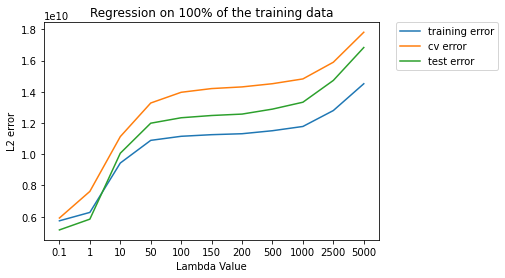
\includegraphics[scale=0.5, angle=0]{templates/1_2_2}
            \caption{Plot showing $\lambda$ and cross-validation loss.}
            \label{fig:my_label}
        \end{figure}
        
        \begin{verbatim}
            lambda:  0.1  
            b:  -1727.2134438706562
            w: [ [-1.33350946e+03]
                 [-5.25444158e+03]
                 [ 1.50281613e+03]
                 [-3.44638514e+01]
                 [ 1.52907091e+02]
                 [-3.01196974e+01]
                 [ 1.15840351e+02]
                 [ 4.78933125e+04]]
            training error 5736263552.429791
            test error 5152682299.804243
            val error 6672178868.376767
        \end{verbatim}
        
        
        \item \textbf{Comparison of models learned by two methods}  For each of the two training sets considered above (5$\%$ and 100$\%$), compare the training and test errors of the models learned using ridge regression. What can you conclude from this about the value of regularization for small and large training sets?
        
        100\% dataset:
        \begin{verbatim}
            training error 5.74e9
            test error 5.15e9
        \end{verbatim}
        
        5\% dataset:
        \begin{verbatim}
            training error 4.42e9
            test error 8.02e9
        \end{verbatim}
        
        On the small training set, training error is lower but test error is much higher. This points to the fact that the regularization parameter is effective in preventing overfitting in large datasets, but not as effective in smaller datasets.
        
        \item \textbf{Theoretical Value of $\lambda$.} For each of the two training sets considered above (5$\%$ and 100$\%$), Which $\lambda$ should be larger by theory?why? Do those values align with the conclusion you made in part 1.3?
        
        As the size of the dataset grows, the size of the optimal $\lambda$ should shrink, in-line with theory.
    
    \end{enumerate}